\chapter{METHODOLOGY}
\section{Modifying the Testing Framework}
The framework of the study is divided into two parts. First, we expand the QoS Testing Framework (hereby referred to as the \textit{simulator}) from Regencia and Yu to support different classes of topologies: fat-tree topologies with fanout greater than 2, some typical topology shapes, general graphs, and data from the Internet Topology Zoo that follow the constraints in section 1.5. Second, we simulate artificial network load with the same methodology as the Regencia and Yu study onto the newly implemented topologies with the same queue management algorithms. 

To accomplish this, we modify the way the \textit{topology configuration} file is read in the Framework. In the original Framework, the topology configuration file contains information about the number of clients and the number of layers in a tree topology, which is then used by each of the \textit{configuration generator} files to reconstruct the topology within itself to generate the correct configuration (Figure \ref{fig:original_architecture}). 

We modify the Framework such that an intermediary script called the \textit{Topology Information Generator} contains the implementation of the topology (Figure \ref{fig:new_architecture}). The Topology Information Generator then can emit a Topology Information file that can be read by the configuration generators to generate the necessary configuration files. For typical topologies such as fat-trees, mesh, and rings, the implementation of the topology is directly in the topology information generator. For topologies from the Internet Topology Zoo data, the generator parses a GraphML file with the  \textsc{NetworkX} library to generate the same information file.

\begin{figure}[htbp!]
    \centering
    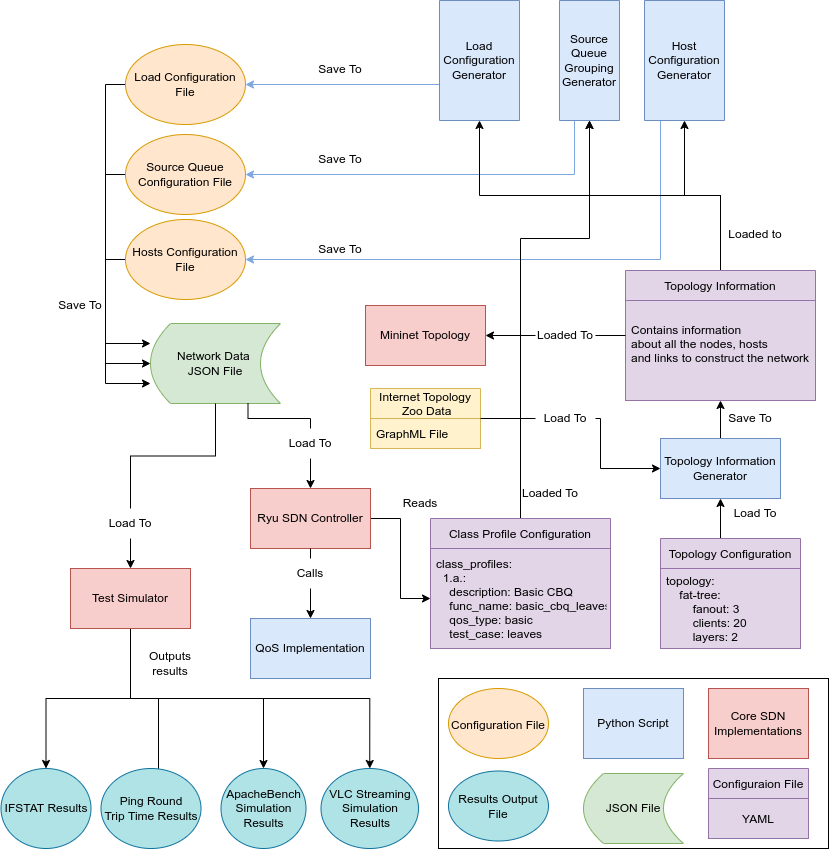
\includegraphics[width=\textwidth]{Figures/Test Framework Architecture.drawio.png}
    \caption{The architecture of the Modified QoS Testing Framework}
    \label{fig:new_architecture}
\end{figure}

The framework is further modified so that the Ryu Controller script now uses the STP protocol to decide the paths of the packets in the topologies, since typical topologies like the mesh and real-life data from the ITZ contain loops for better network resiliency \cite{smith_shortest_2011}. The reference \textsc{simple\_switch\_stp\_13.py} code from the Ryu Library is used as a basis to develop the controller that will run on any topology and with any QoS queue management technique.

Finally, we simplify the framework so that the framework no longer needs pickle files to specify the QoS Implementations. Instead, the Ryu Controller directly calls the appropriate QoS Implementation according to the algorithm specified by the \textit{Class Profile Configuration} file. The modified framework is installed on a system configured as described in Figure \ref{fig:tools}. Software in the \textit{SDN Simulation} box are used for simulating the networks and running the tests, while the tools in the \textit{Topology Processing} box are used for selecting, diagramming, and processing the various topologies.

\begin{figure}[htbp]
    \centering
    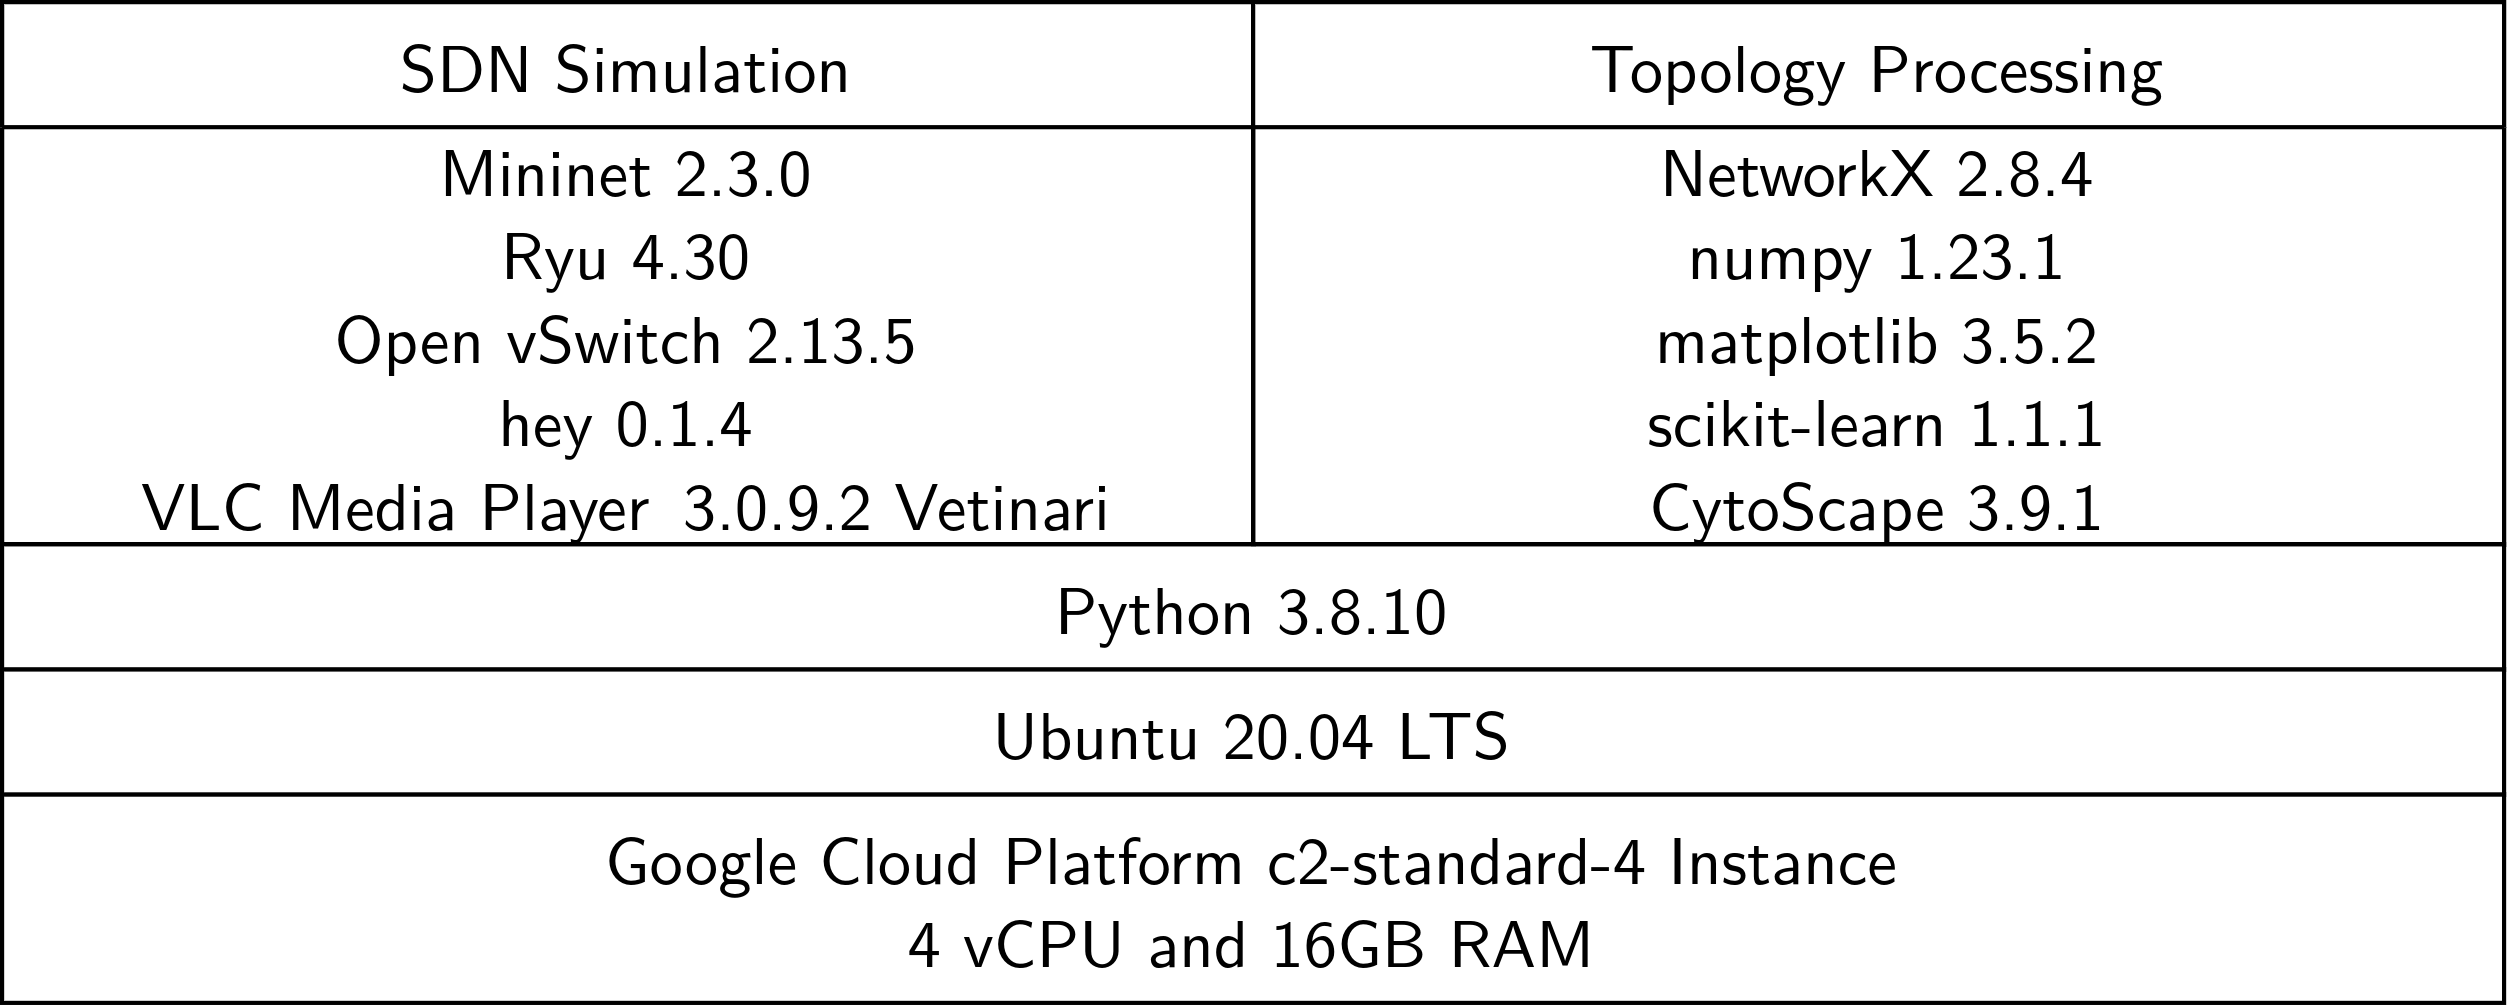
\includegraphics[width=\textwidth]{Figures/Test Machine Configuration.drawio.png}
    \caption{The machine configuration and software tools used in the experiment}
    \label{fig:tools}
\end{figure}

\section{Selected Networks for Testing}
We test the following topologies:
\begin{enumerate}
    \item Fat-tree topology with two layers and fan-out 3 (Figure \ref{fig:BalancedTree})
    \item Hypercube topology with 8 vertices (Figure \ref{fig:Hypercube})
    \item Complete Mesh topology with 5 vertices in the mesh (Figure \ref{fig:CompleteMesh})
    \item Topology from the Internet Topology Zoo, Regional or Country data with less than 40 nodes
\end{enumerate}

The choice of topologies from the Internet Topology Zoo is based on two features: the number of nodes and the number of edges (links) in the graph. From the dataset in the ITZ, we have 133 topologies that are either regional or country data that has less than 40 nodes. This limit is due to the limited resources of the machine that runs the simulations. The clustering was done by reading all 133 topologies into NetworkX, extracting the number of nodes and edges, and using the \textsc{scikit-learn} KMeans clustering library. Each node-edge data point was given the same weight \cite{scikit-learn}. Centroid selection seed was fixed as $0$. We chose 10 random topologies from the four clusters with NumPy, proportional to the number of topologies in each group. The list of the chosen topologies are shown in Table \ref{tab:choices}.

\begin{figure}[htbp]
    \centering
    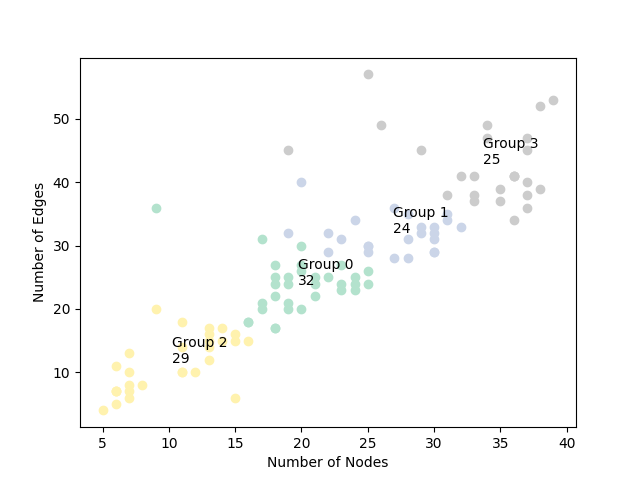
\includegraphics[width=\textwidth]{Figures/clusters.png}
    \caption{133 ITZ topologies as grouped by K-means method based on the number of nodes and number of edges. Numbers in the middle of similarly-colored points indicate the number of topologies in the group.}
    \label{fig:groups}
\end{figure}

\begin{table}[htbp]
    \centering
    \begin{tabular}{ccccc}
    \toprule
        Topology Name & Cluster & \makecell{Number of\\ Nodes} & \makecell{Number of \\Edges} & Location \\
    \midrule
        Saavis (Figure \ref{fig:Saavis}) & 0 & 19 & 20 & USA \\
        Atmnet (Figure \ref{fig:Atmnet})& 0 & 21 & 22 & USA \\
        Ibm (Figure \ref{fig:Ibm})& 0 & 18 & 24 & USA \\
        Agis (Figure \ref{fig:Agis})& 1 & 25 & 30 & USA \\
        WideJpn (Figure \ref{fig:WideJpn})& 1 & 30 & 33 & Japan \\
        Gridnet (Figure \ref{fig:Gridnet})& 2 & 9 & 20 & USA \\
        Nsfnet (Figure \ref{fig:Nsfnet})& 2 & 13 & 15 & USA \\
        Singaren (Figure \ref{fig:Singaren})& 2 & 11 & 10 & Singapore \\
        Janetbackbone (Figure \ref{fig:Janetbackbone})& 3 & 29 & 45 & UK \\
        Canerie (Figure \ref{fig:Canerie})& 3 & 32 & 41 & Canada \\
    \bottomrule
    \end{tabular}
    \caption{10 topologies from the 4 clusters chosen at random with NumPy. Diagrams for these networks are in Appendix I.}
    \label{tab:choices}
\end{table}

In general, we have selected topologies of various sizes, some with many loops, and some with structures that are more tree-like. Although this only simulates networks with less than 40 nodes, the variety of network structure and sizes are still evident in the samples.

\section{Topology Configuration}
To implement the topologies within the context of the simulations, we take the fat-tree topology from the original study by Regencia and Yu and modify the number, arrangement, and links in the switches that connect the ``core'' switch to the clients. The ``core'' switch is the switch that connects to a switch connecting all servers in a star topology formation. In Figure \ref{fig:original_topology}, the topology to be changed corresponds to the circled switches.

\begin{figure}[htbp]
    \centering
    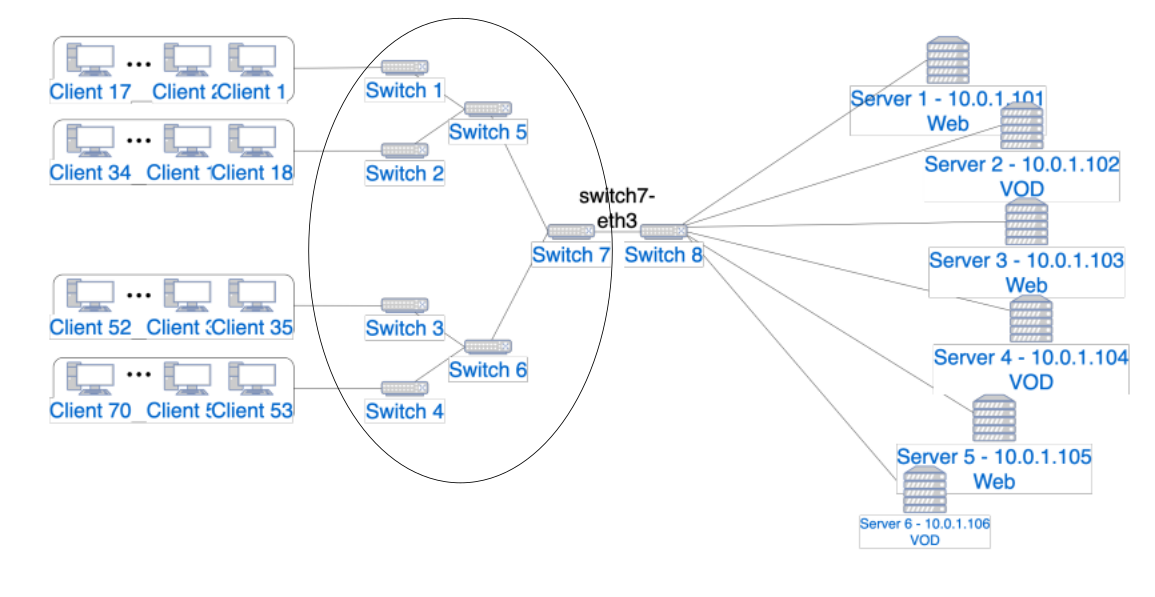
\includegraphics[width=\textwidth]{Figures/original_topology.png}
    \caption{Diagram of a fat-tree topology tested in Regencia and Yu}
    \label{fig:original_topology}
\end{figure}

The ``core'' switch in the fat-tree topology remains to be the root switch of the tree. In the complete mesh topology and the hypercube, the node with the numerical label $0$ is considered to be the root switch, since the topologies has at least one symmetry with respect to any node in the mesh. For the topologies from the Internet Topology Zoo, we simulate the worst case scenario by assigning the core as the node with the highest number of total hops from all other nodes, which is calculated with the Floyd-Warshall algorithm provided by the NetworkX library.

Clients are placed on all ``leaf'' switches, or switches furthest away from the ``core'' switch, which are switches that have the longest path from the core switch in the graph that represents the topology. As an exception, the fat-tree topology will have clients connected to its explicit leaf switches. The clients will be distributed equally among the switches. Finally, we will connect four servers to the server switch to complete the topology. The diagrams of the tested topologies are included in Appendix I.

Links will be configured with their default setting of 10Gbps in Mininet, as in the previous study. Although real-life networks do not behave this way, the ITZ data is not complete to simulate the link speeds.

\section{Server Configuration}
There will be 2 servers running a Python server from the http.server library, and 2 servers running a VLC streaming server using the Real Time Streaming Protocol. Table \ref{tab:httpserverconfig} shows the files hosted by the HTTP servers, and Table \ref{tab:vlcconfig} shows the videos hosted by the VLC servers.

\begin{table}[htbp]
    \centering
    \begin{tabular}{cccc}
        \toprule
        \multirow{2}{*}{Server ID} & \multirow{2}{*}{Server IP Address} & \multicolumn{2}{c}{File Size and Type} \\
         &  & Low Load & High Load \\
        \midrule
        Server 1 & 10.0.1.101 & \qty{100}{\kilo \byte} JPEG & \qty{10}{\mega \byte} JPEG \\
        Server 3 & 10.0.1.103 & \qty{16}{\mega \byte} PDF & \qty{100}{\mega \byte} PDF  \\
        \bottomrule
    \end{tabular}
    \caption{Files hosted by the two Python http.server servers}
    \label{tab:httpserverconfig}
\end{table}

\begin{table}[htbp]
    \centering
    \begin{tabular}{cccc}
        \toprule
        \multirow{2}{*}{Server ID} & \multirow{2}{*}{Server IP Address} & \multicolumn{2}{c}{Video Resolution} \\
         &  & Low Load & High Load \\
        \midrule
        Server 2 & 10.0.1.102 & 360p & 480p \\
        Server 4 & 10.0.1.104 & 480p & 720p  \\
        \bottomrule
    \end{tabular}
    \caption{Files hosted by the two VLC RTSP servers}
    \label{tab:vlcconfig}
\end{table}

\section{Client Configuration}
There will be 48 clients that will simultaneously run an ApacheBenchmark test and a VLC client. Each client will request for different files from the server, and every file in each server will get requests as equally as possible. Table \ref{tab:clientconfig} shows the configuration of these clients.

\begin{table}[htbp]
    \centering
    \begin{tabular}{ccc}
    \toprule
        Client numbers & Server & Load\\
    \midrule
        \multirow{2}{*}{$1, 5, 9, 13, \dots 41, 45$}  & Server 1 & Low \\
        & Server 2 & Low \\ \hline
        \multirow{2}{*}{$2, 6, 10, 14, \dots 42, 46$}  & Server 3 & Low \\
        & Server 4 & Low \\ \hline
        \multirow{2}{*}{$3, 7, 11, 15, \dots 43, 47$}  & Server 1 & High \\
        & Server 2 & High \\ \hline
        \multirow{2}{*}{$4, 8, 12, 16, \dots 44, 48$}  & Server 3 & High \\
        & Server 4 & High \\
    \bottomrule
    \end{tabular}
    \caption{Configurations for clients denoting the server and the load that the client will request in the simulations}
    \label{tab:clientconfig}
\end{table}

\section{Quality of Service configuration}
The parameters for QoS Ports are identical to the configuration in Regencia and Yu. In the case of leaf-enforced QoS, the parameters will be applied to all ports at the switches that are connected to the clients. In the case of core-enforced QoS, they will be applied at the port connecting the core switch to the server switch. Table \ref{tab:qosconfig} shows the configuration used for this study.

\begin{table}[htbp]
    \centering
    \begin{tabular}{cccc}
    \toprule
        Queue number & Type of traffic & \thead{Minimum and \\Maximum bandwidth} & Priority\\
    \midrule
        $Q_0$ & TCP & \qty{333.33}{\mega \bit / \second} & 1 \\
        $Q_1$ & UDP & \qty{333.33}{\mega \bit / \second} & 2 \\
        $Q_2$ & Others(ICMP, ARP) & \qty{333.33}{\mega \bit / \second} & 0 \\
    \bottomrule
    \end{tabular}
    \caption{Configurations used for ports where QoS parameters are enforced}
    \label{tab:qosconfig}
\end{table}


\section{Network Simulation and Testing}
The methodology of testing the networks is similar to Chato and Yu \cite{chato_exploration_2016} which is also used in Regencia and Yu \cite{yang_introducing_2022}. Since the modified framework uses STP, we have to wait for the STP to converge before running the rest of the tests. We first run pings until a successful ping has been executed. We measure the time for this to take for all topologies. Then, for the actual tests, we wait for at least this amount of time before executing the rest of the tests.

For every topology, we run ping tests, IFSTAT, ApacheBenchmark, and VLC Streaming under all the QoS algorithms to be tested. We show the exact process of running the benchmarks in Figure \ref{fig:benchmark}.

\begin{figure}
    \centering
    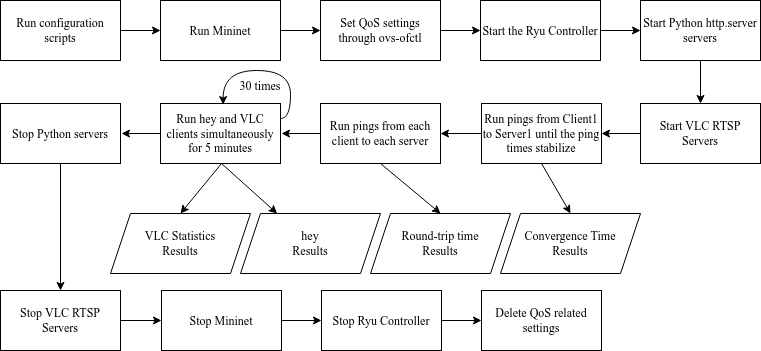
\includegraphics[width=\textwidth]{Figures/Test Procedure.drawio.png}
    \caption{The procedure for running the benchmarks}
    \label{fig:benchmark}
\end{figure}

One key difference between this methodology and the methodology from Regencia and Yu is that different topologies take different amounts of time for the switches in the network to install flows. We define the \textit{convergence time} as the time it takes for pings to go consistently under 1 second after the STP established proper connections between the servers and the clients. Yoo and Yu have shown that the convergence time is different for different types of topologies \cite{yoo_building_2022}. Therefore, this characteristic is measured first before running other tests.
